\subsubsection{NASA-TLX}
\label{subsubsec:results_nasa_tlx_2}

\paragraph{Analysis of the mental demand scale}\mbox{}\\

Table \ref{tab:md_table_noBase} presents the mental demand score of all participants, while the corresponding barplot is presented in Figure \ref{fig:barplot_md_avg_4_scene_blind_sight}. As said before, the higher the value, the higher is the mental demand of the user. It is interesting to observe that sighted people gave a higher score to audio, as they are not so familiar with using sounds as source of guidance.


\begin{table}[!htb]
\centering
\caption{Mental demand felled by the participants.}
\label{tab:md_table_noBase}
\begin{tabular}{lllrrrrr}
\toprule
    &       &        & Audio & \begin{tabular}[c]{@{}l@{}}Haptic\\ Belt\end{tabular} & \begin{tabular}[c]{@{}l@{}}Virtual\\ Cane\end{tabular} & Mixture \\
Participant & \begin{tabular}[c]{@{}l@{}}Visual\\ Condition\end{tabular} & Round &       &                                                       &                                                        &         \\
\midrule
001 & Sight & First &    12 &                                                    11 &                                                      5 &       9 \\
    &       & Return &    13 &                                                    13 &                                                      5 &      10 \\
001C & Blind & First &     1 &                                                    14 &                                                      3 &       6 \\
    &       & Return &     1 &                                                    10 &                                                      2 &       6 \\
002C & Blind & First &     1 &                                                     1 &                                                     10 &      12 \\
    &       & Return &     1 &                                                     1 &                                                     10 &       3 \\
003 & Sight & First &    18 &                                                    18 &                                                     16 &      10 \\
    &       & Return &    12 &                                                    15 &                                                     11 &       8 \\
003C & Blind & First &     5 &                                                     5 &                                                      8 &       1 \\
    &       & Return &     1 &                                                     1 &                                                      2 &       1 \\
004 & Sight & First &    17 &                                                    20 &                                                     12 &      20 \\
    &       & Return &    12 &                                                    15 &                                                     10 &      15 \\
004C & Blind & First &    10 &                                                    15 &                                                     10 &      10 \\
    &       & Return &    10 &                                                    14 &                                                      8 &      10 \\
005 & Sight & First &     4 &                                                    12 &                                                     10 &      13 \\
    &       & Return &     6 &                                                    10 &                                                      6 &      12 \\
\bottomrule
\end{tabular}
\end{table}



\begin{figure}[!thb]
    \centering
    \begin{minipage}{\textwidth}
        \centering
        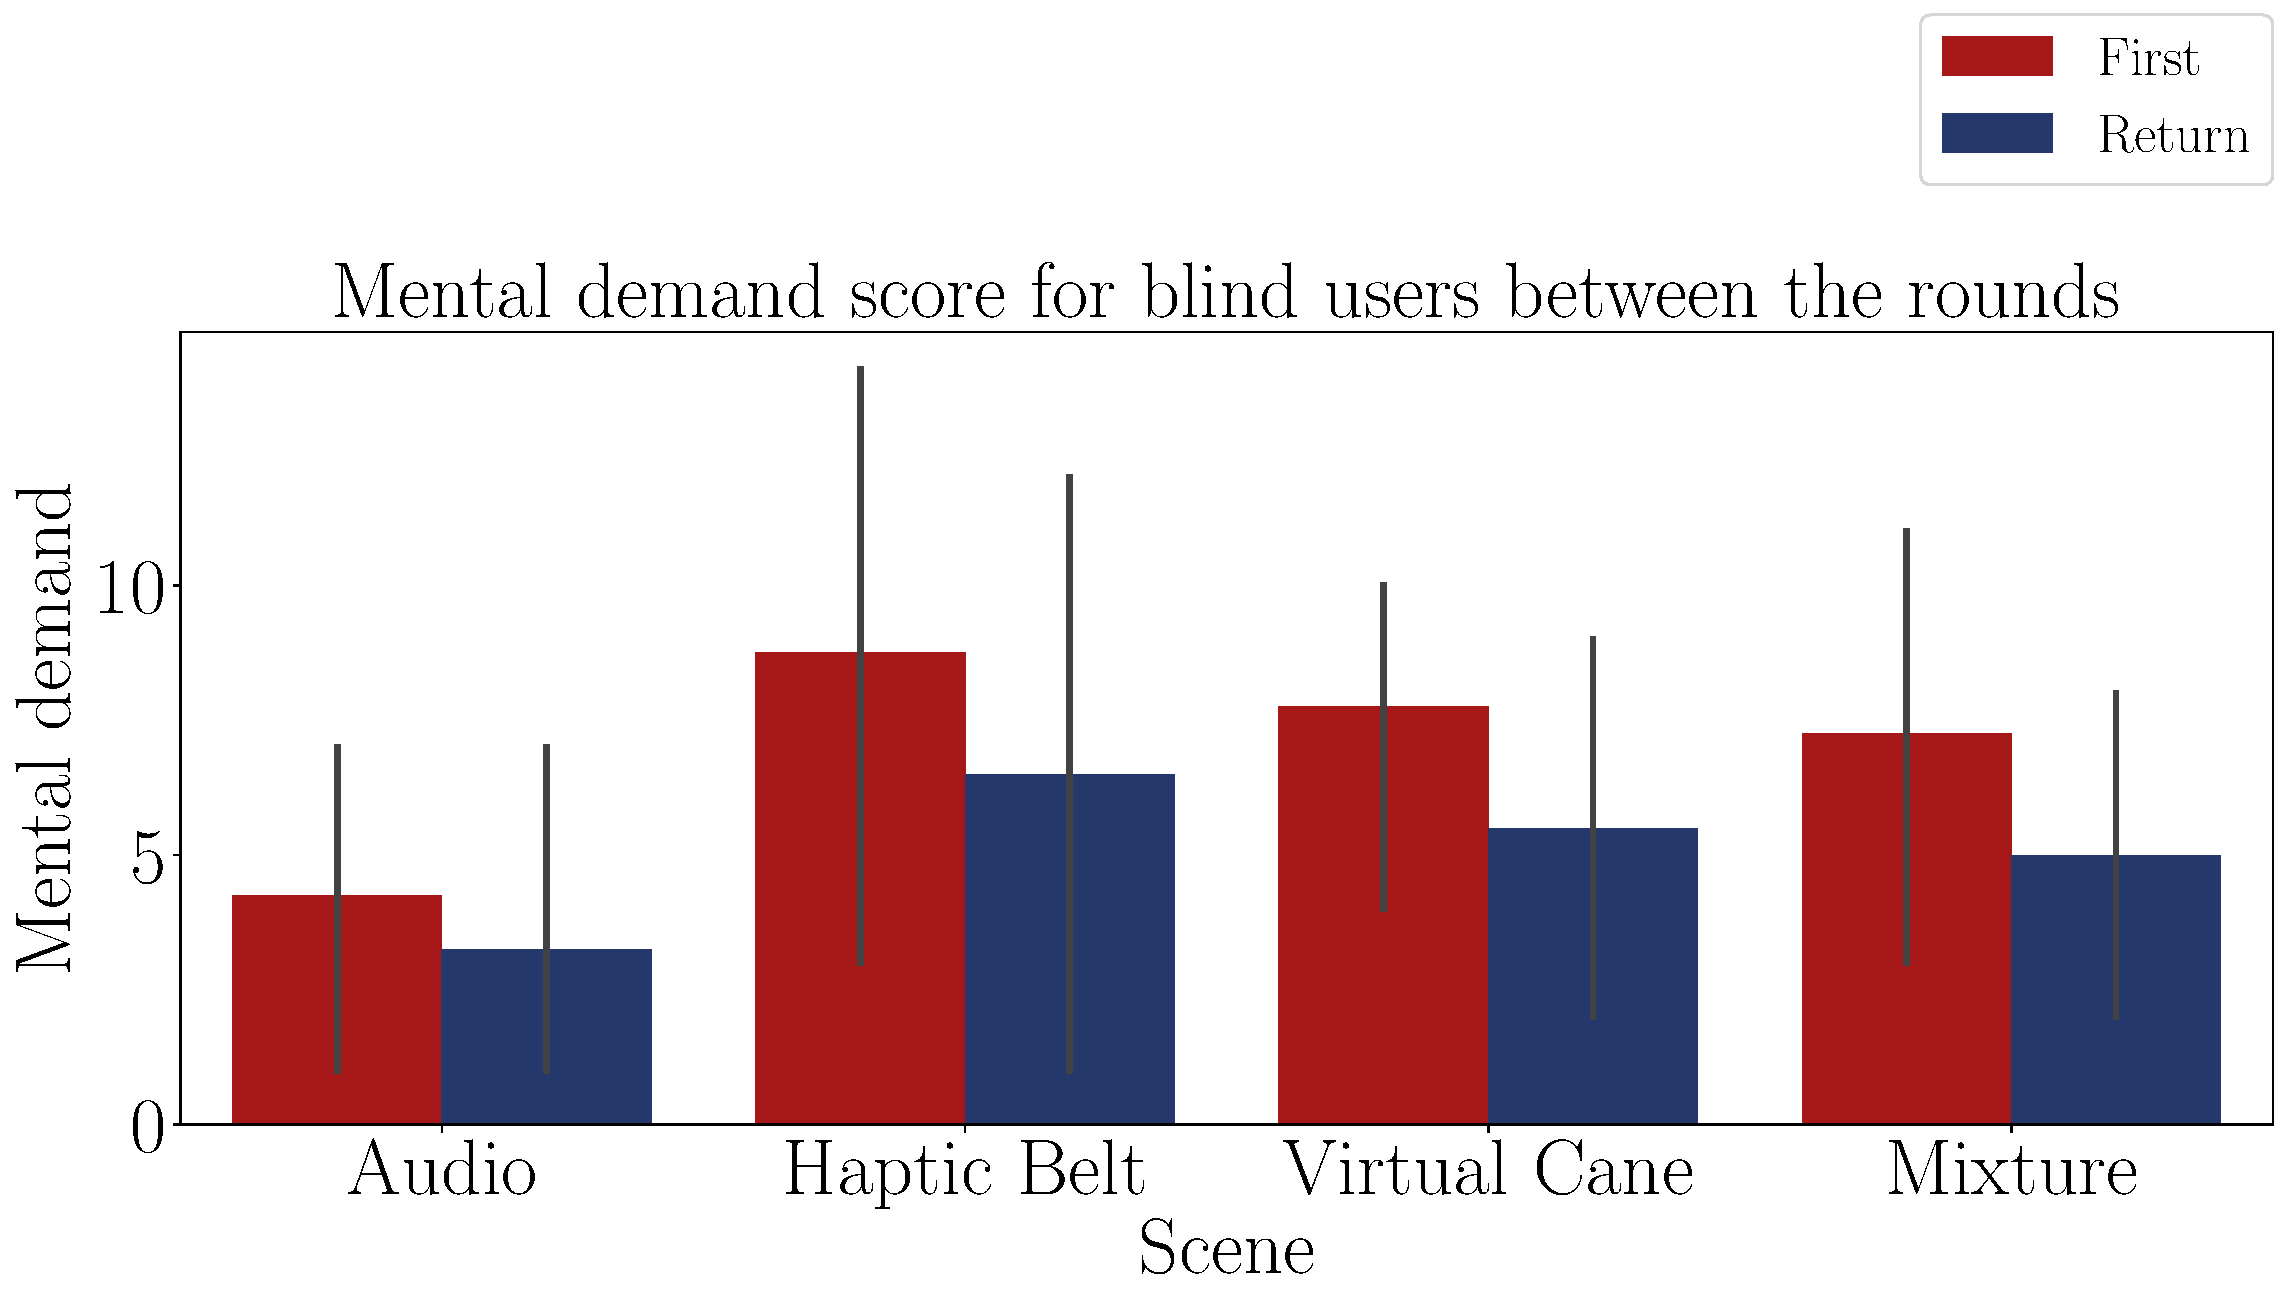
\includegraphics[width = \textwidth]{Resultados/Nasa/Figuras/pdf/barplot_md_avg_4_scene_blind.pdf}
        \subcaption{Blind participants}
        \label{fig:barplot_md_avg_4_scene_blind}
    \end{minipage}
    \begin{minipage}{\textwidth}
        \centering
        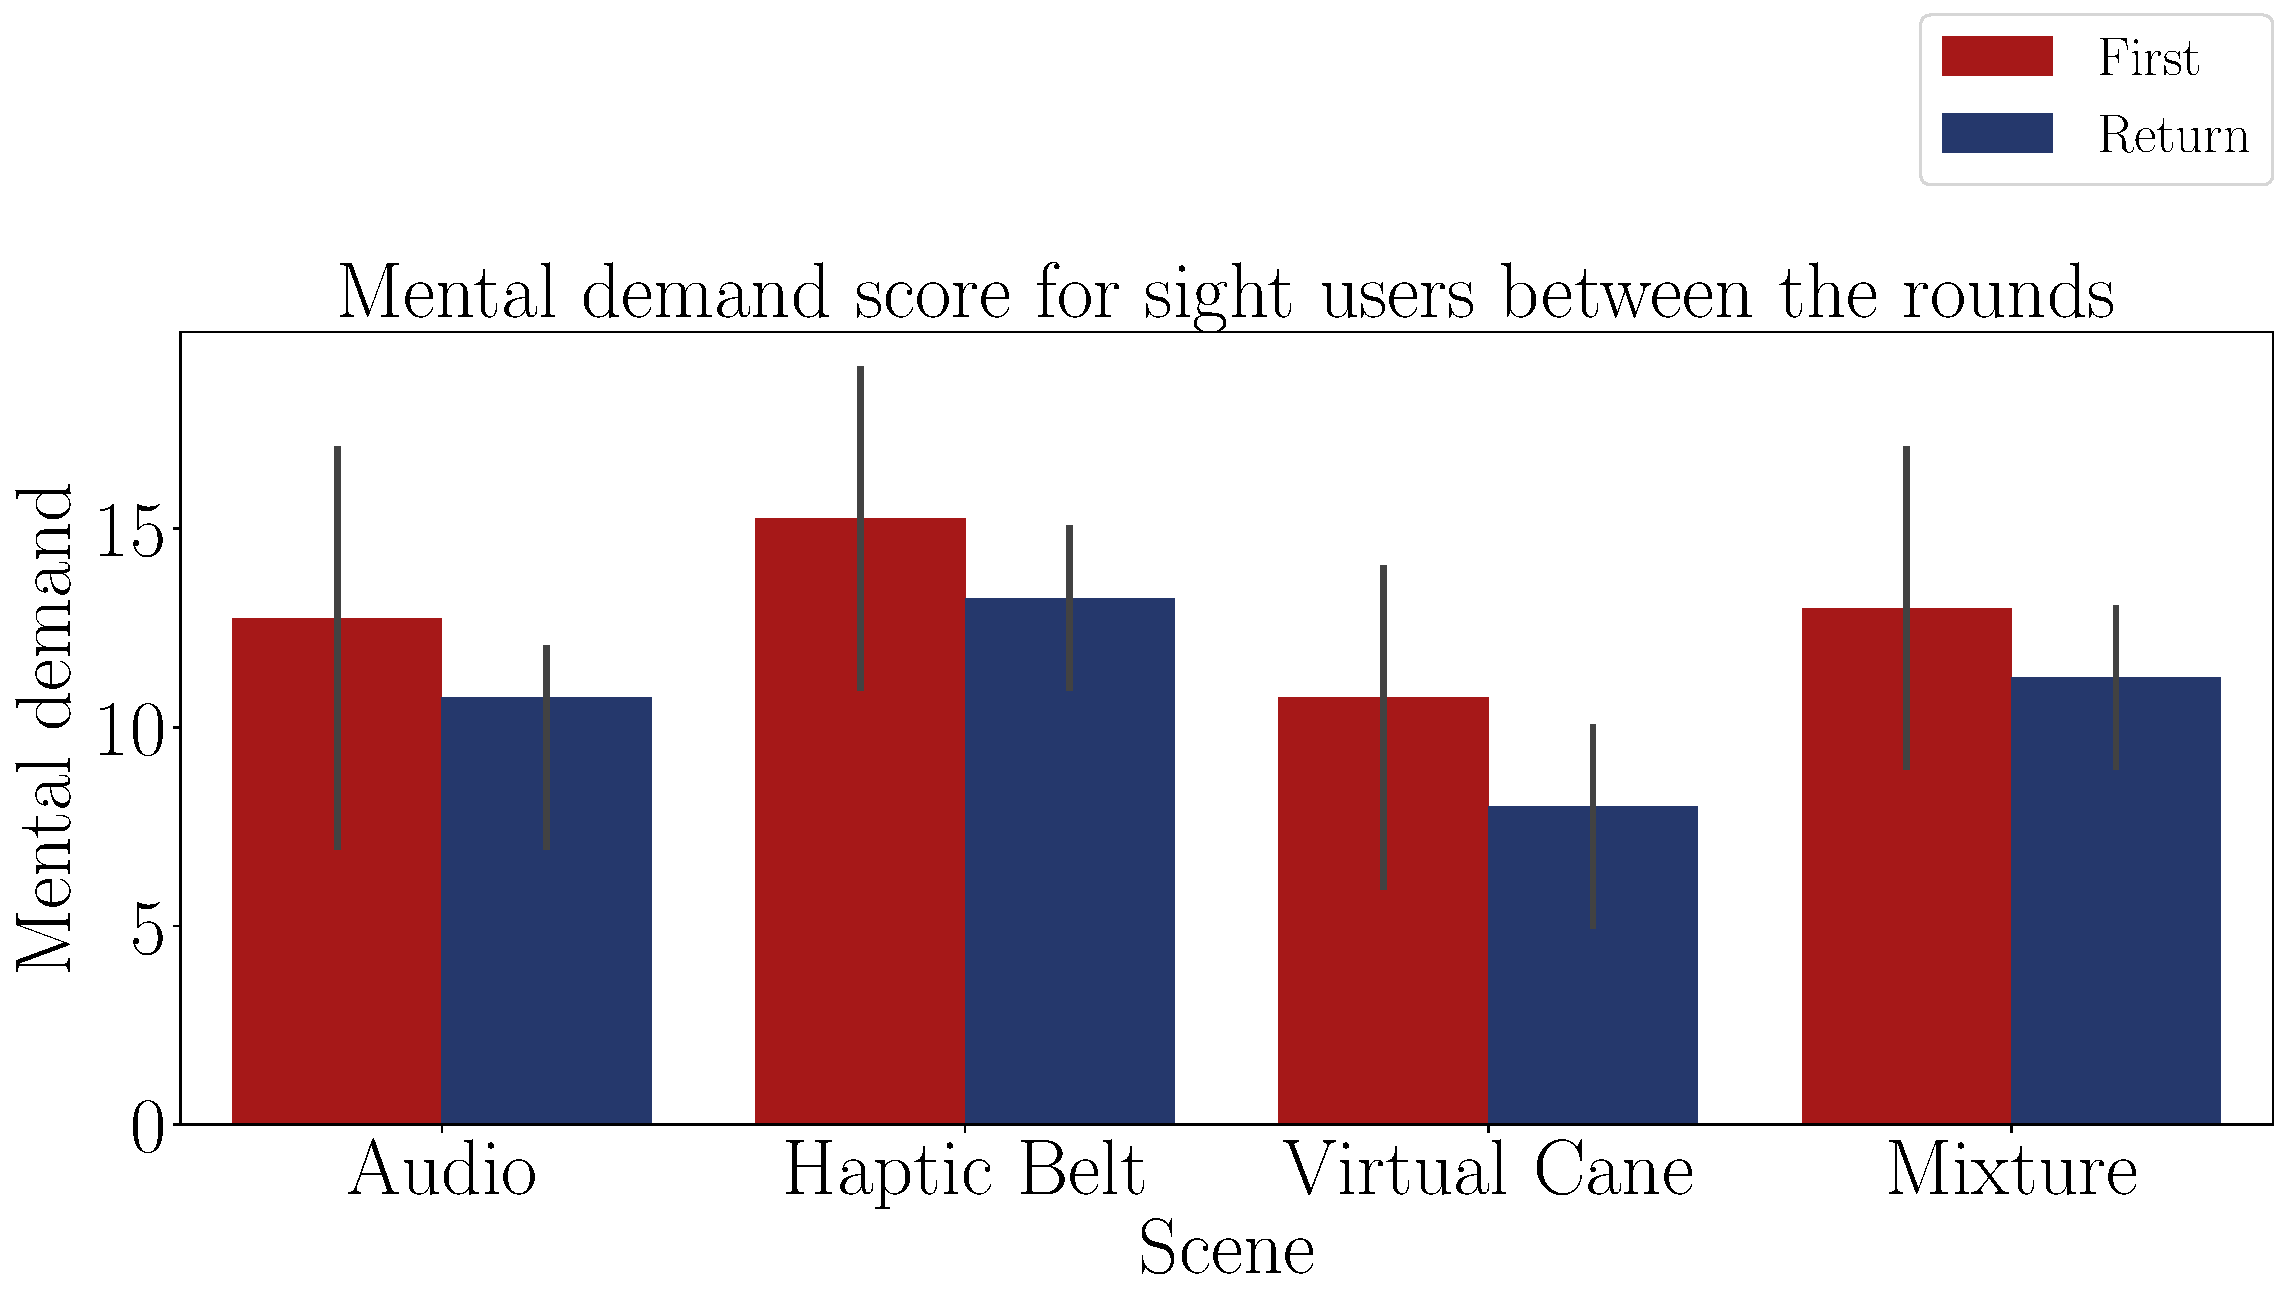
\includegraphics[width = \textwidth]{Resultados/Nasa/Figuras/pdf/barplot_md_avg_4_scene_sight.pdf}
        \subcaption{Sight participants}
        \label{fig:barplot_md_avg_4_scene_sight}
    \end{minipage}
    \caption{Barplot of the average mental demand on each method and each round.}
    \label{fig:barplot_md_avg_4_scene_blind_sight}
\end{figure}

Figures \ref{fig:boxplot_noBase_md_4_scene} and \ref{fig:boxplot_noBase_md_4_rounds} presents the box plot for both groups, organized by the methods and the rounds. The mental demand is systematically higher for sighted people, which is expected. However, while blind participants considered the audio method less demanding, sighted participants prefered to the virtual cane. For both groups, we observe a decrease in the mental demand.

\begin{figure}[!htb]
    \centering
    \begin{minipage}{0.45\textwidth}
        \centering
        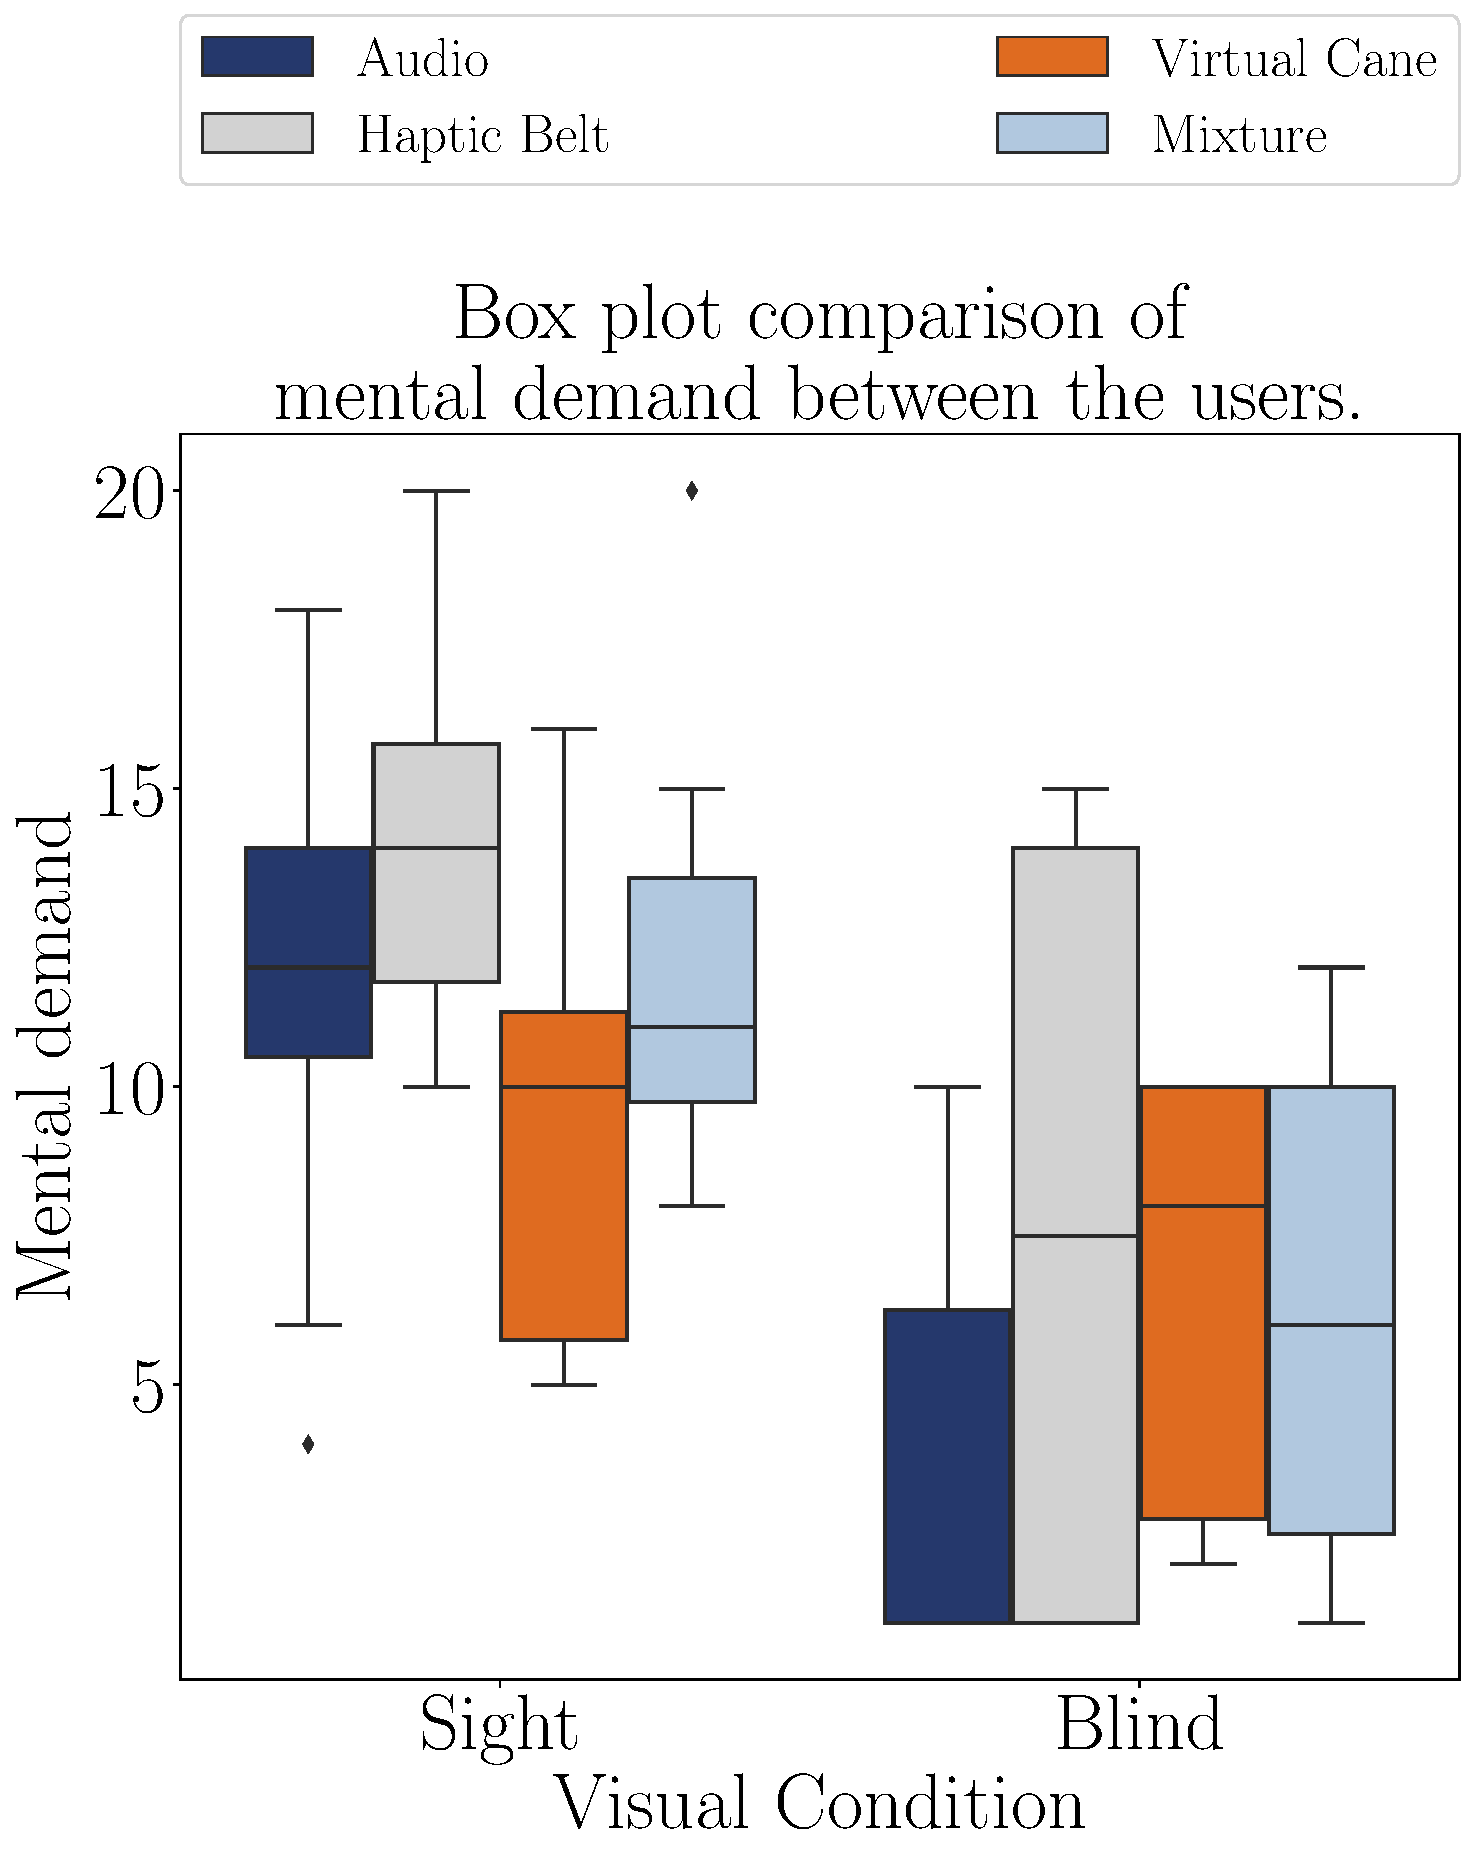
\includegraphics[width = \textwidth]{Resultados/Nasa/Figuras/pdf/boxplot_noBase_md_4_scene.pdf}
        \caption{Boxplot of the mental demand of the participants grouped by the methods.}
        \label{fig:boxplot_noBase_md_4_scene}
    \end{minipage}
    \begin{minipage}{0.075\textwidth}
        \hfill
    \end{minipage}
    \begin{minipage}{0.45\textwidth}
        \centering
        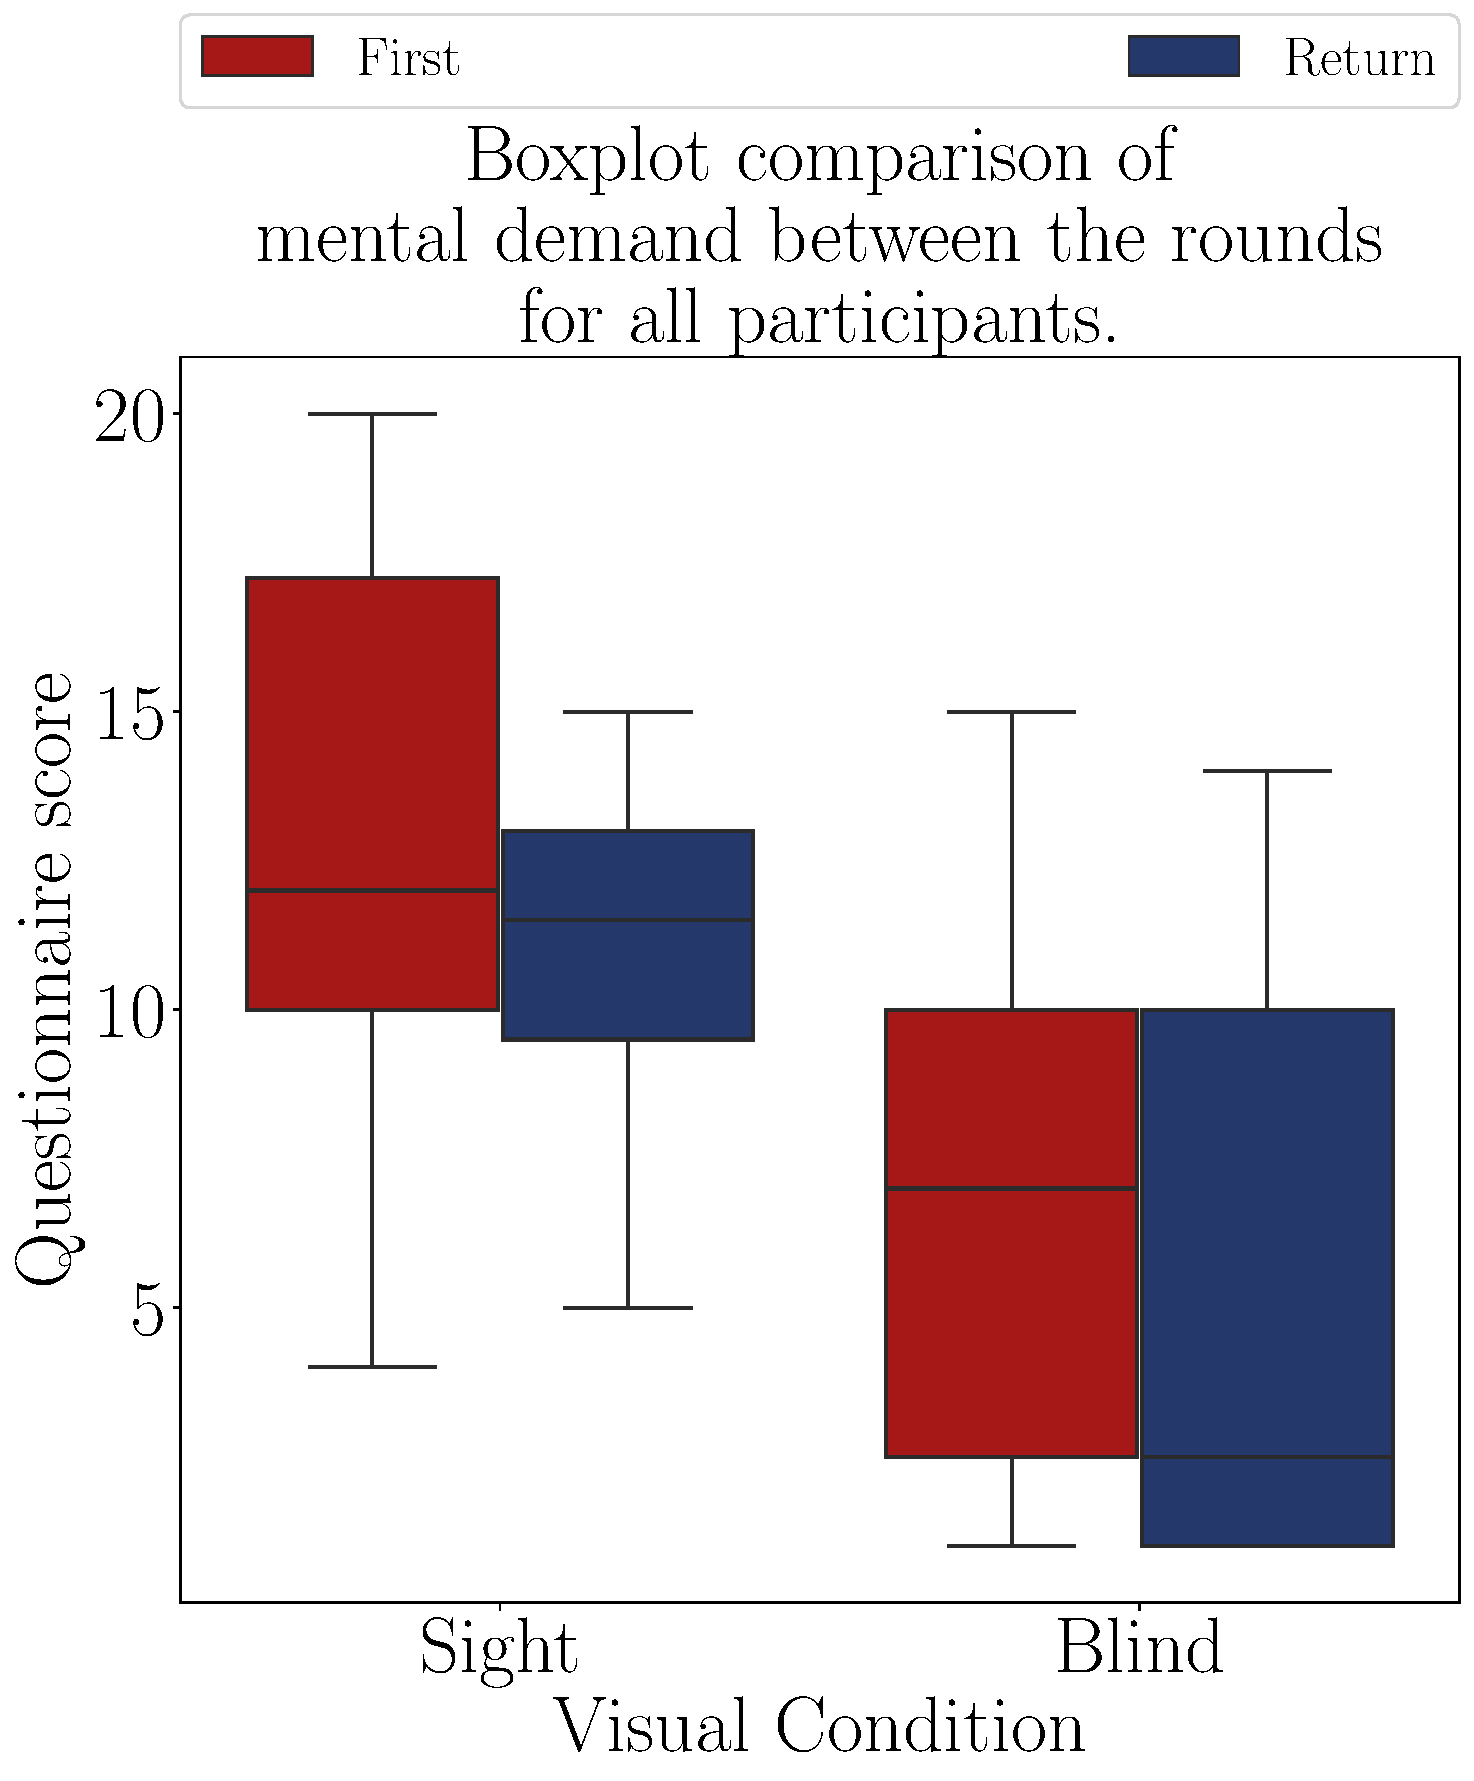
\includegraphics[width = \textwidth]{Resultados/Nasa/Figuras/pdf/boxplot_noBase_md_4_rounds.pdf}
        \caption{Boxplot of the mental demand of the participants grouped by the rounds.}
        \label{fig:boxplot_noBase_md_4_rounds}
    \end{minipage}
\end{figure}

Figures \ref{fig:qqplot_md_avg_two_way_sight} and \ref{fig:residplot_md_avg_two_way_sight} show the QQ plot and residual distribution for the sighted data, confirming that the data is normally distributed and participants have similar variance. Table \ref{tab:blocanova_md_avg_two_way_blind_sight} brings the results of ANOVA. Unlike the blind participants, in the case of sighted ones, the p-value for the methods is below the threshold of 0.05, confirming it as a significant variable for the mental demand. In the case of the rounds, the data from both sighted and blind participants resulted in the exact p-value of 0.075, which is close to the traditional threshold of 0.05 but slightly higher. 

\begin{table}[!htb]
    \caption{Anova p-value for the mental demand average on each method'}
    \label{tab:blocanova_md_avg_two_way_blind_sight}
\begin{minipage}{0.45\textwidth}
    \subcaption{Blind participants}
    
\centering
\begin{tabular}{ll}
\toprule
          Source & P-Value \\
\midrule
    \    Methods &   0.170 \\
     \    Rounds &   0.075 \\
\    Interaction &   0.993 \\
\bottomrule
\end{tabular}

\end{minipage}
\begin{minipage}{0.45\textwidth}
    \subcaption{Sight participants}
    
\centering
\begin{tabular}{ll}
\toprule
          Source & P-Value \\
\midrule
    \    Methods & 0.049** \\
     \    Rounds &   0.075 \\
\    Interaction &   0.990 \\
\bottomrule
\end{tabular}
    
\end{minipage}
\end{table}

\begin{figure}[!htb]
    \centering
    %\vspace{-15.0cm}
    \begin{minipage}{0.45\textwidth}
        \centering
        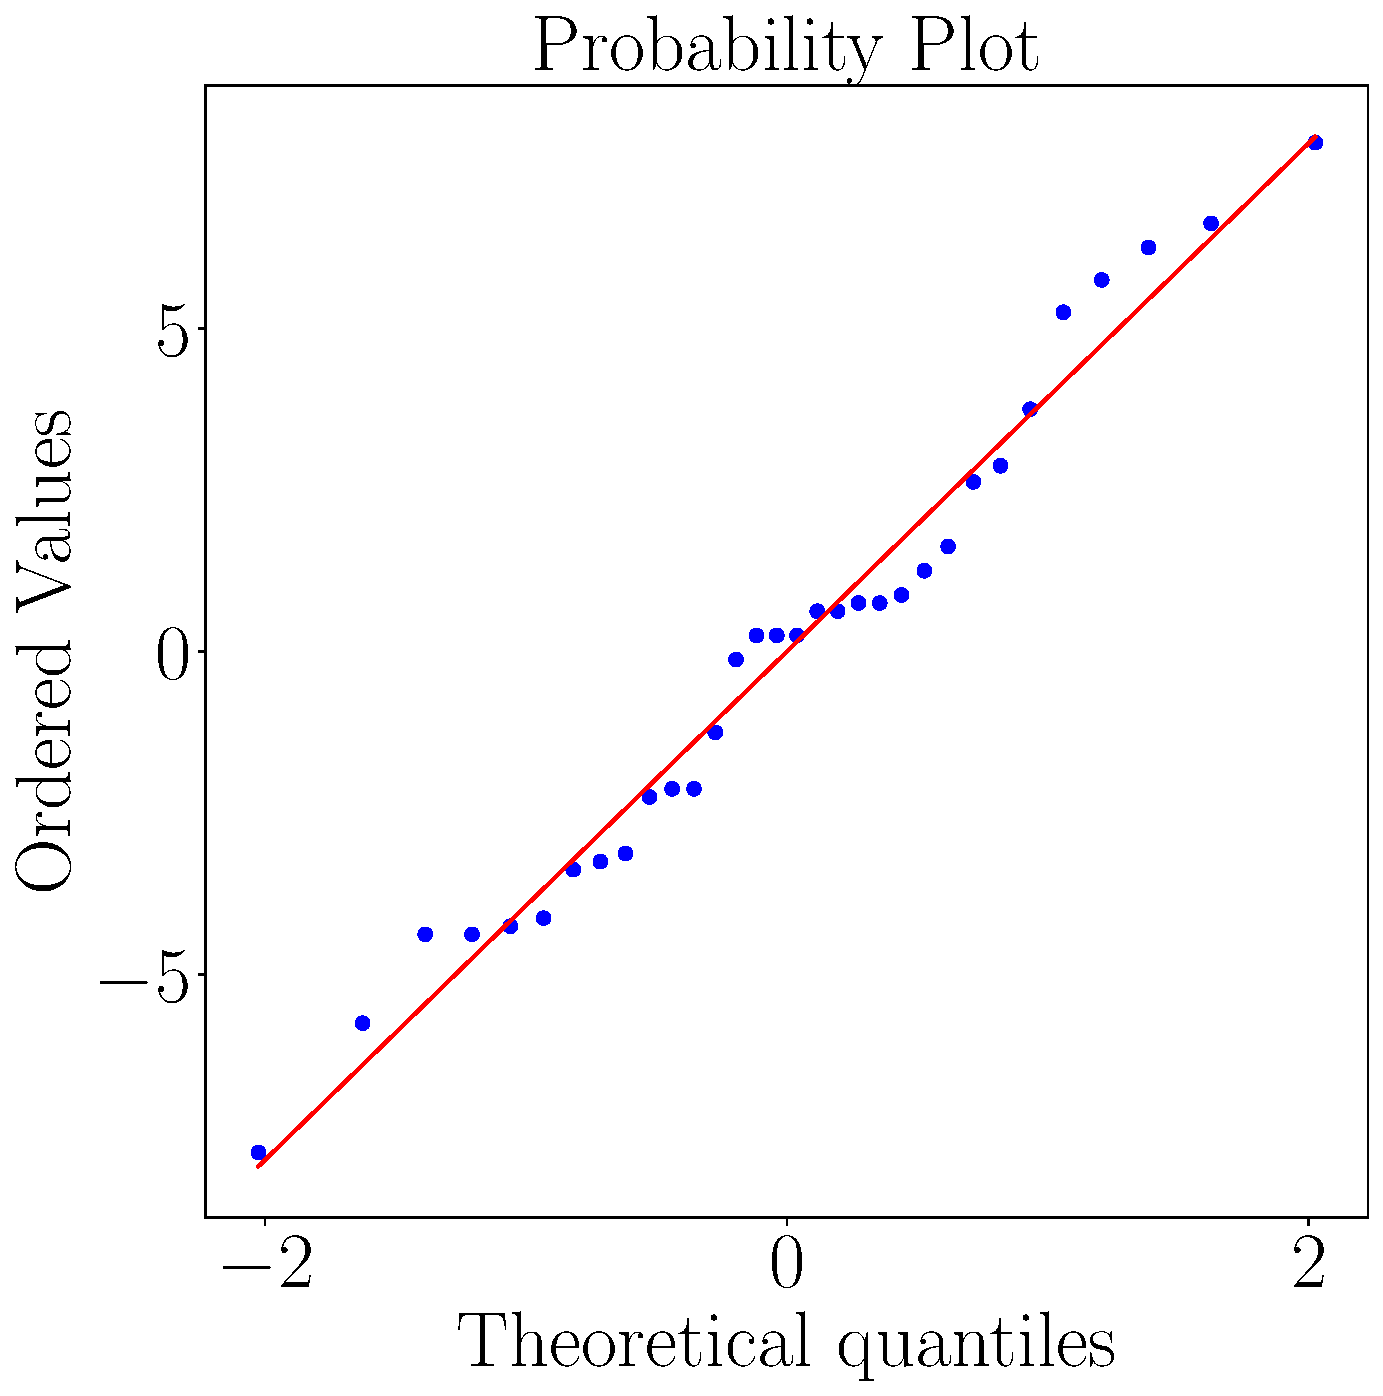
\includegraphics[width = \textwidth]{Resultados/Nasa/Figuras/pdf/qqplot_md_avg_two_way_sight.pdf}
        \caption{QQ plot of the mental demand of the sight participants on each method.}
        \label{fig:qqplot_md_avg_two_way_sight}
    \end{minipage}
    \begin{minipage}{0.075\textwidth}
        \hfill
    \end{minipage}
    \begin{minipage}{0.45\textwidth}
        \centering
        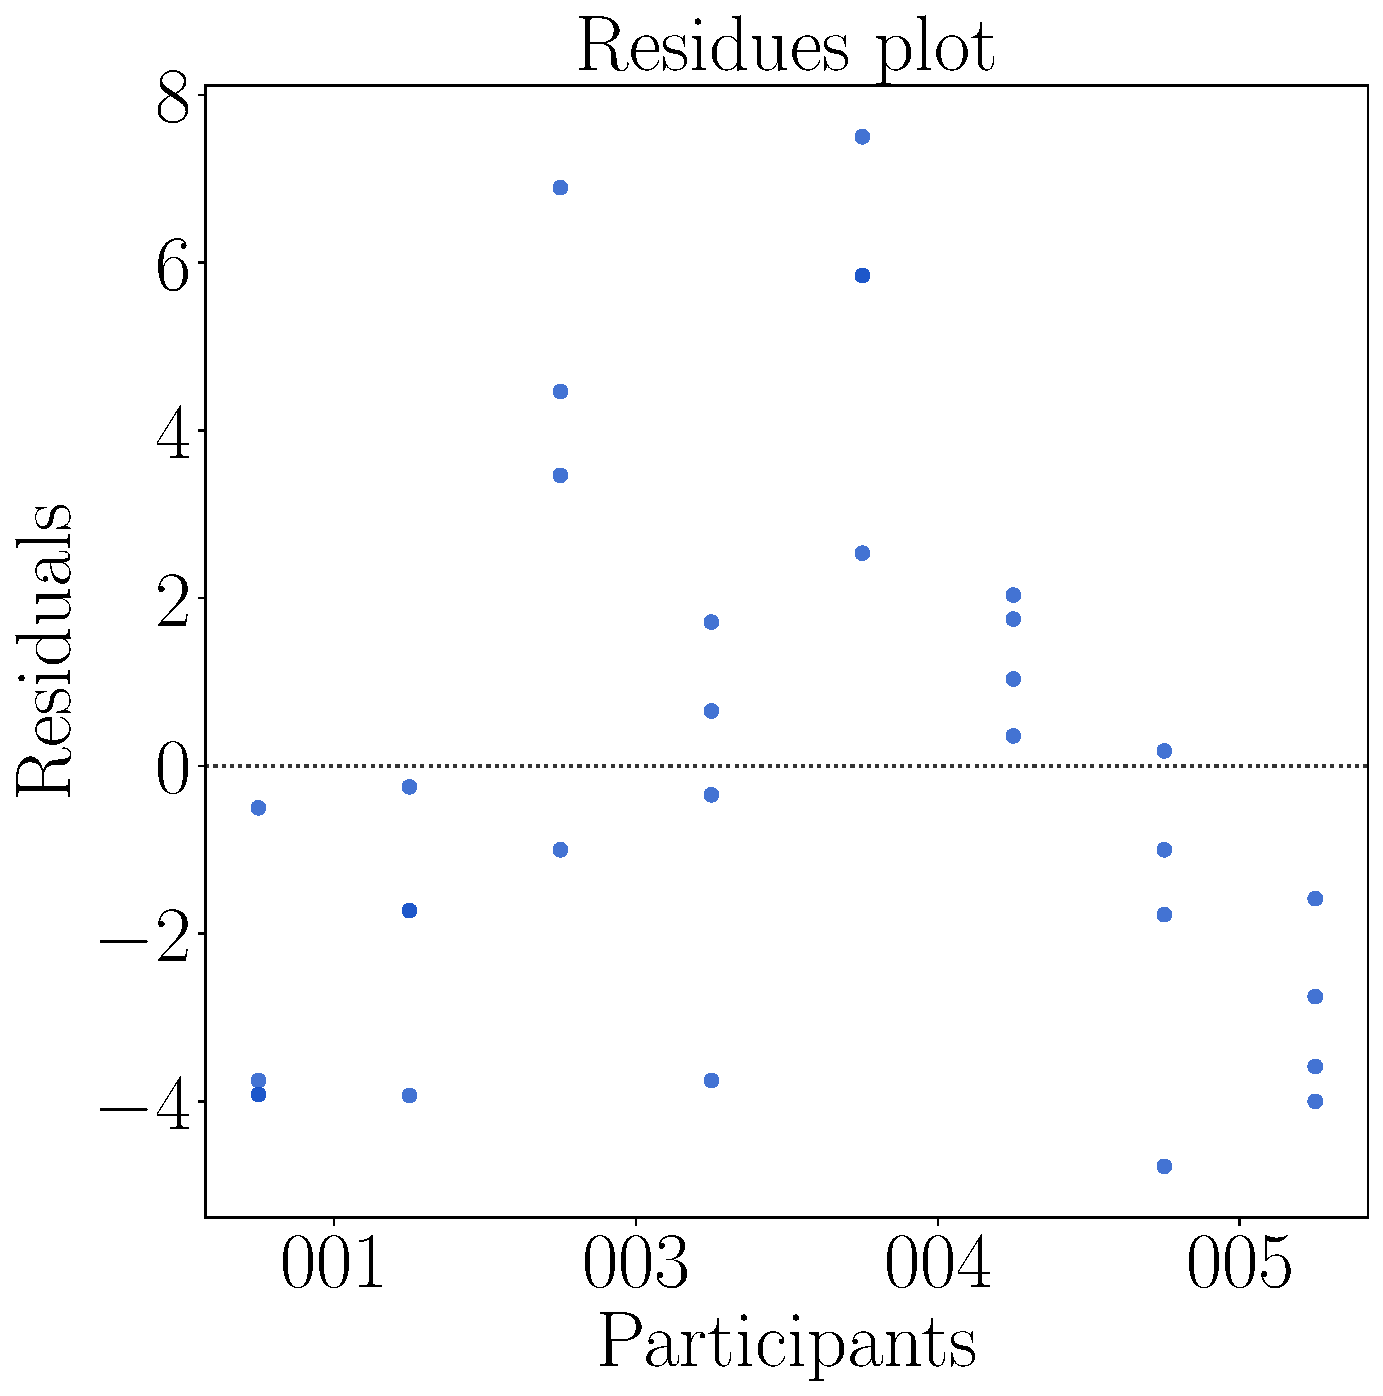
\includegraphics[width = \textwidth]{Resultados/Nasa/Figuras/pdf/residplot_md_avg_two_way_sight.pdf}
        \caption{Residual plot of the mental demand score the sighted participants on each method.}
        \label{fig:residplot_md_avg_two_way_sight}
    \end{minipage}
\end{figure}

\FloatBarrier

%%%%%%%%%%%%%%%%%%%%%%%%%%%%%%%%%%%%%%%%%%%%%%%%%%%%%%%%%%%%%%%%%%%%%%%%%%%%
%%%%%%%%%%%%%%%%%%%%%%%%%%%%%%%%%%%%%%%%%%%%%%%%%%%%%%%%%%%%%%%%%%%%%%%%%%%%
%%%%%%%%%%%%%%%%%%%%%%%%%%%%%%%%%%%%%%%%%%%%%%%%%%%%%%%%%%%%%%%%%%%%%%%%%%%%
%%%%%%%%%%%%%%%%%%%%%%%%%%%%%%%%%%%%%%%%%%%%%%%%%%%%%%%%%%%%%%%%%%%%%%%%%%%%


\paragraph{Analysis of the NASA-TLX score}\mbox{}\\

Table \ref{tab:nasa_table_noBase} brings the NASA-TLX global score of all participants, while the corresponding barplot is presented in Figure \ref{fig:barplot_nasa_avg_4_scene}. As before, the higher the value, the higher is the Mental Workload of the user.


\begin{table}[!htb]
\centering
\caption{NASA-TLX score felled by the participants.}
\label{tab:nasa_table_noBase}
\begin{tabular}{lllrrrrr}
\toprule
    &       &        &  Audio & \begin{tabular}[c]{@{}l@{}}Haptic\\ Belt\end{tabular} & \begin{tabular}[c]{@{}l@{}}Virtual\\ Cane\end{tabular} & Mixture \\
Participant & \begin{tabular}[c]{@{}l@{}}Visual\\ Condition\end{tabular} & Round &        &                                                       &                                                        &         \\
\midrule
001 & Sight & First & 10.167 &                                                 9.833 &                                                  7.000 &   9.000 \\
    &       & Return & 11.000 &                                                10.833 &                                                  6.167 &   9.333 \\
001C & Blind & First &  4.000 &                                                 8.833 &                                                  5.167 &   6.333 \\
    &       & Return &  4.000 &                                                 6.667 &                                                  4.500 &   6.167 \\
002C & Blind & First &  4.833 &                                                 4.833 &                                                  9.000 &   7.000 \\
    &       & Return &  4.833 &                                                 4.833 &                                                  7.000 &   5.167 \\
003 & Sight & First &  9.833 &                                                10.167 &                                                  9.500 &   6.500 \\
    &       & Return &  6.667 &                                                 9.667 &                                                  7.833 &   4.833 \\
003C & Blind & First &  4.000 &                                                 5.333 &                                                  6.667 &   3.500 \\
    &       & Return &  3.833 &                                                 3.667 &                                                  3.500 &   3.500 \\
004 & Sight & First & 14.833 &                                                13.667 &                                                 11.500 &  15.833 \\
    &       & Return & 11.833 &                                                11.833 &                                                 10.833 &  12.167 \\
004C & Blind & First & 10.000 &                                                12.667 &                                                  9.667 &  11.000 \\
    &       & Return &  9.167 &                                                11.667 &                                                  9.333 &  10.833 \\
005 & Sight & First &  7.667 &                                                 9.000 &                                                  8.000 &   9.667 \\
    &       & Return &  7.667 &                                                 8.667 &                                                  7.667 &   6.000 \\
\bottomrule
\end{tabular}
\end{table}



From Figure \ref{fig:barplot_nasa_avg_4_scene}, it is possible to see that, similar to blind participants, sighted participants consider that the workload of the return round was lower than that of the first round. However, similar to what happened for the mental demand, sighted participants considered virtual cane as the methods with the lowest workload, while, for  blind participants, it was the audio.

\begin{figure}[!htb]
    \centering
    \begin{minipage}{\textwidth}
        \centering
        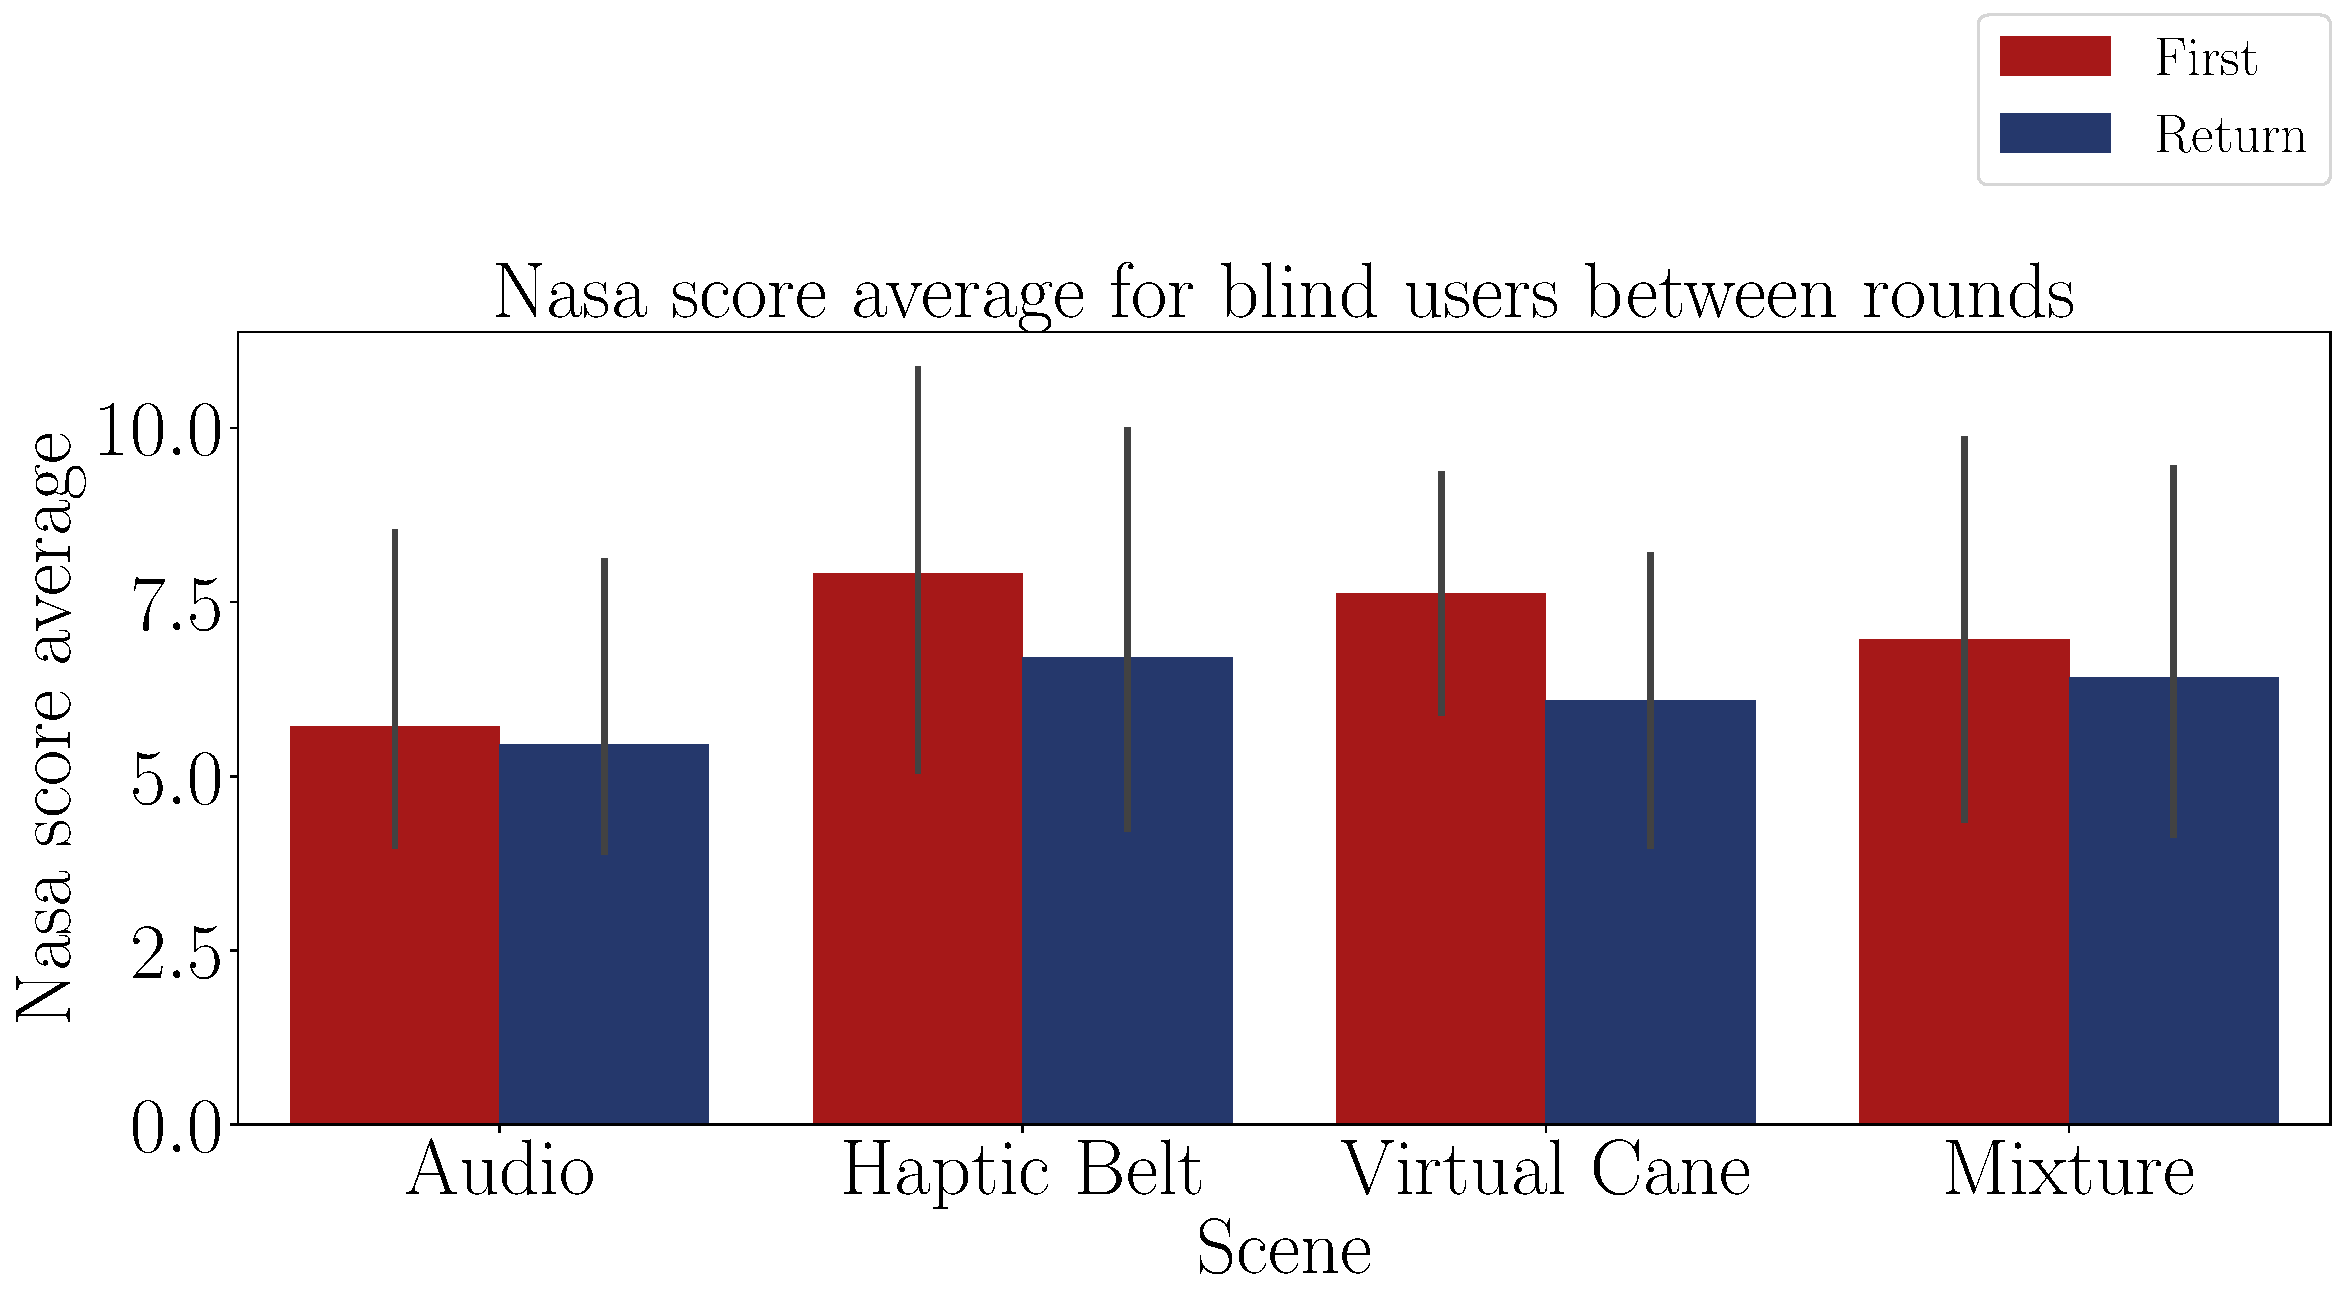
\includegraphics[width = \textwidth]{Resultados/Nasa/Figuras/pdf/barplot_nasa_avg_4_scene_blind.pdf}
        \subcaption{Blind participants.}
        \label{fig:barplot_nasa_avg_4_scene_blind}
    \end{minipage}
    \begin{minipage}{\textwidth}
        \centering
        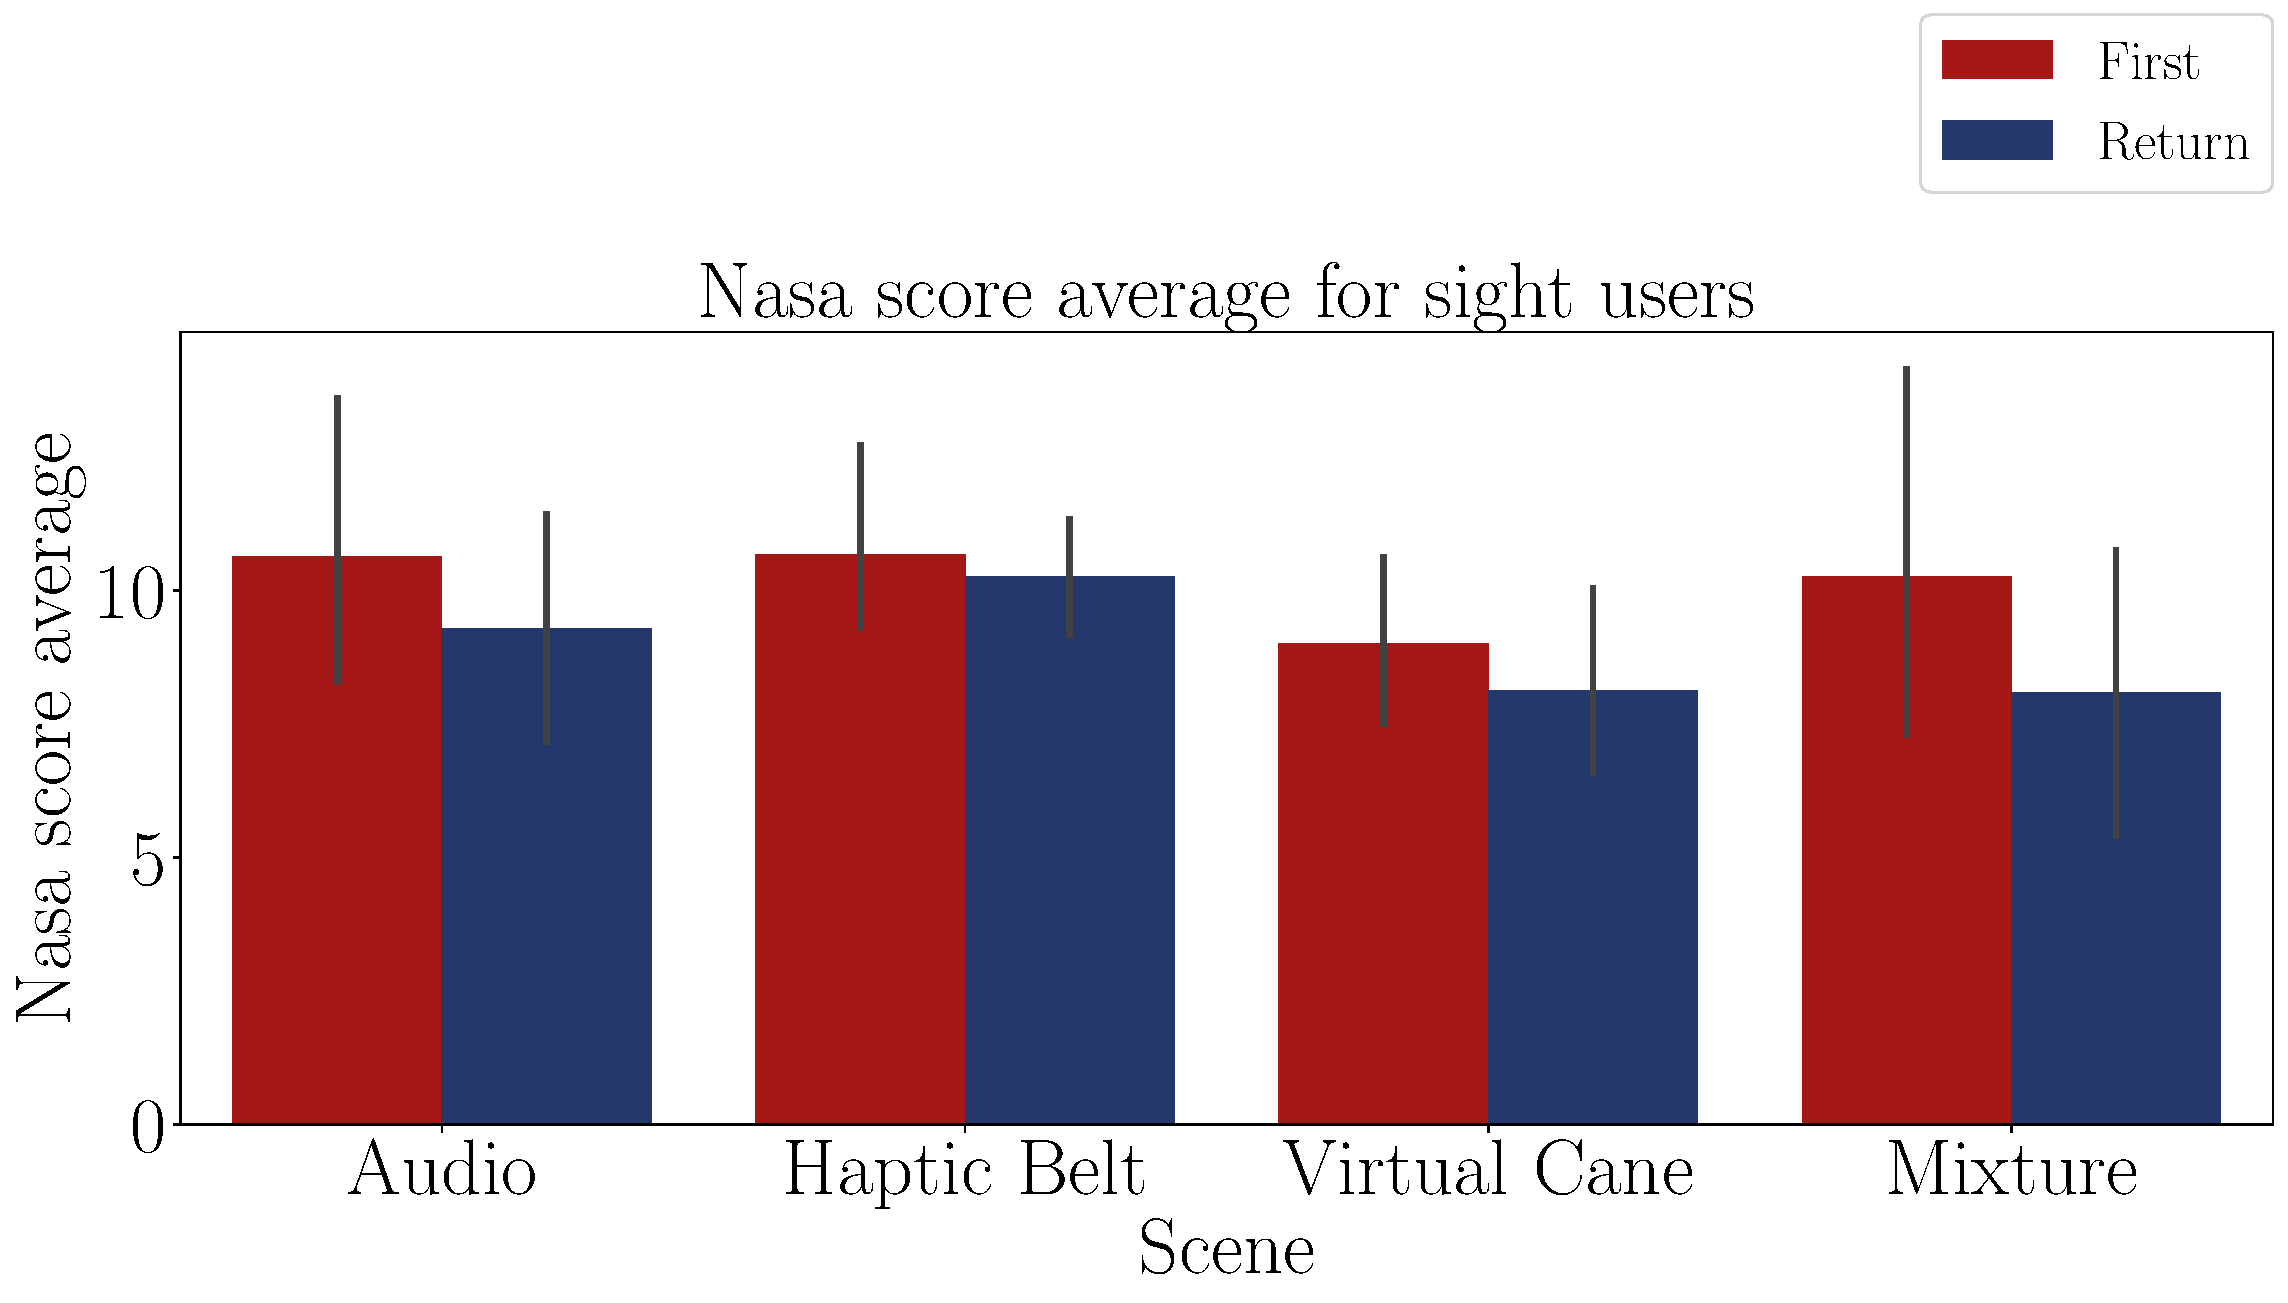
\includegraphics[width = \textwidth]{Resultados/Nasa/Figuras/pdf/barplot_nasa_avg_4_scene_sight.pdf}
        \subcaption{Sight participants.}
        \label{fig:barplot_nasa_avg_4_scene_sight}
    \end{minipage}
    \caption{Barplot of the NASA-TLX score on each method and each round.}
    \label{fig:barplot_nasa_avg_4_scene}
\end{figure}

Figures \ref{fig:boxplot_noBase_nasa_4_scene} and \ref{fig:boxplot_noBase_nasa_4_rounds} present the boxplots of the NASA-TLX global score. Again, it is possible to see that sighted people usually give higher workload scores than blind ones. The influence of the round is approximately the same. However, the order of preference of the methods is different.

\begin{figure}[!htb]
    \centering
    \begin{minipage}{0.45\textwidth}
        \centering
        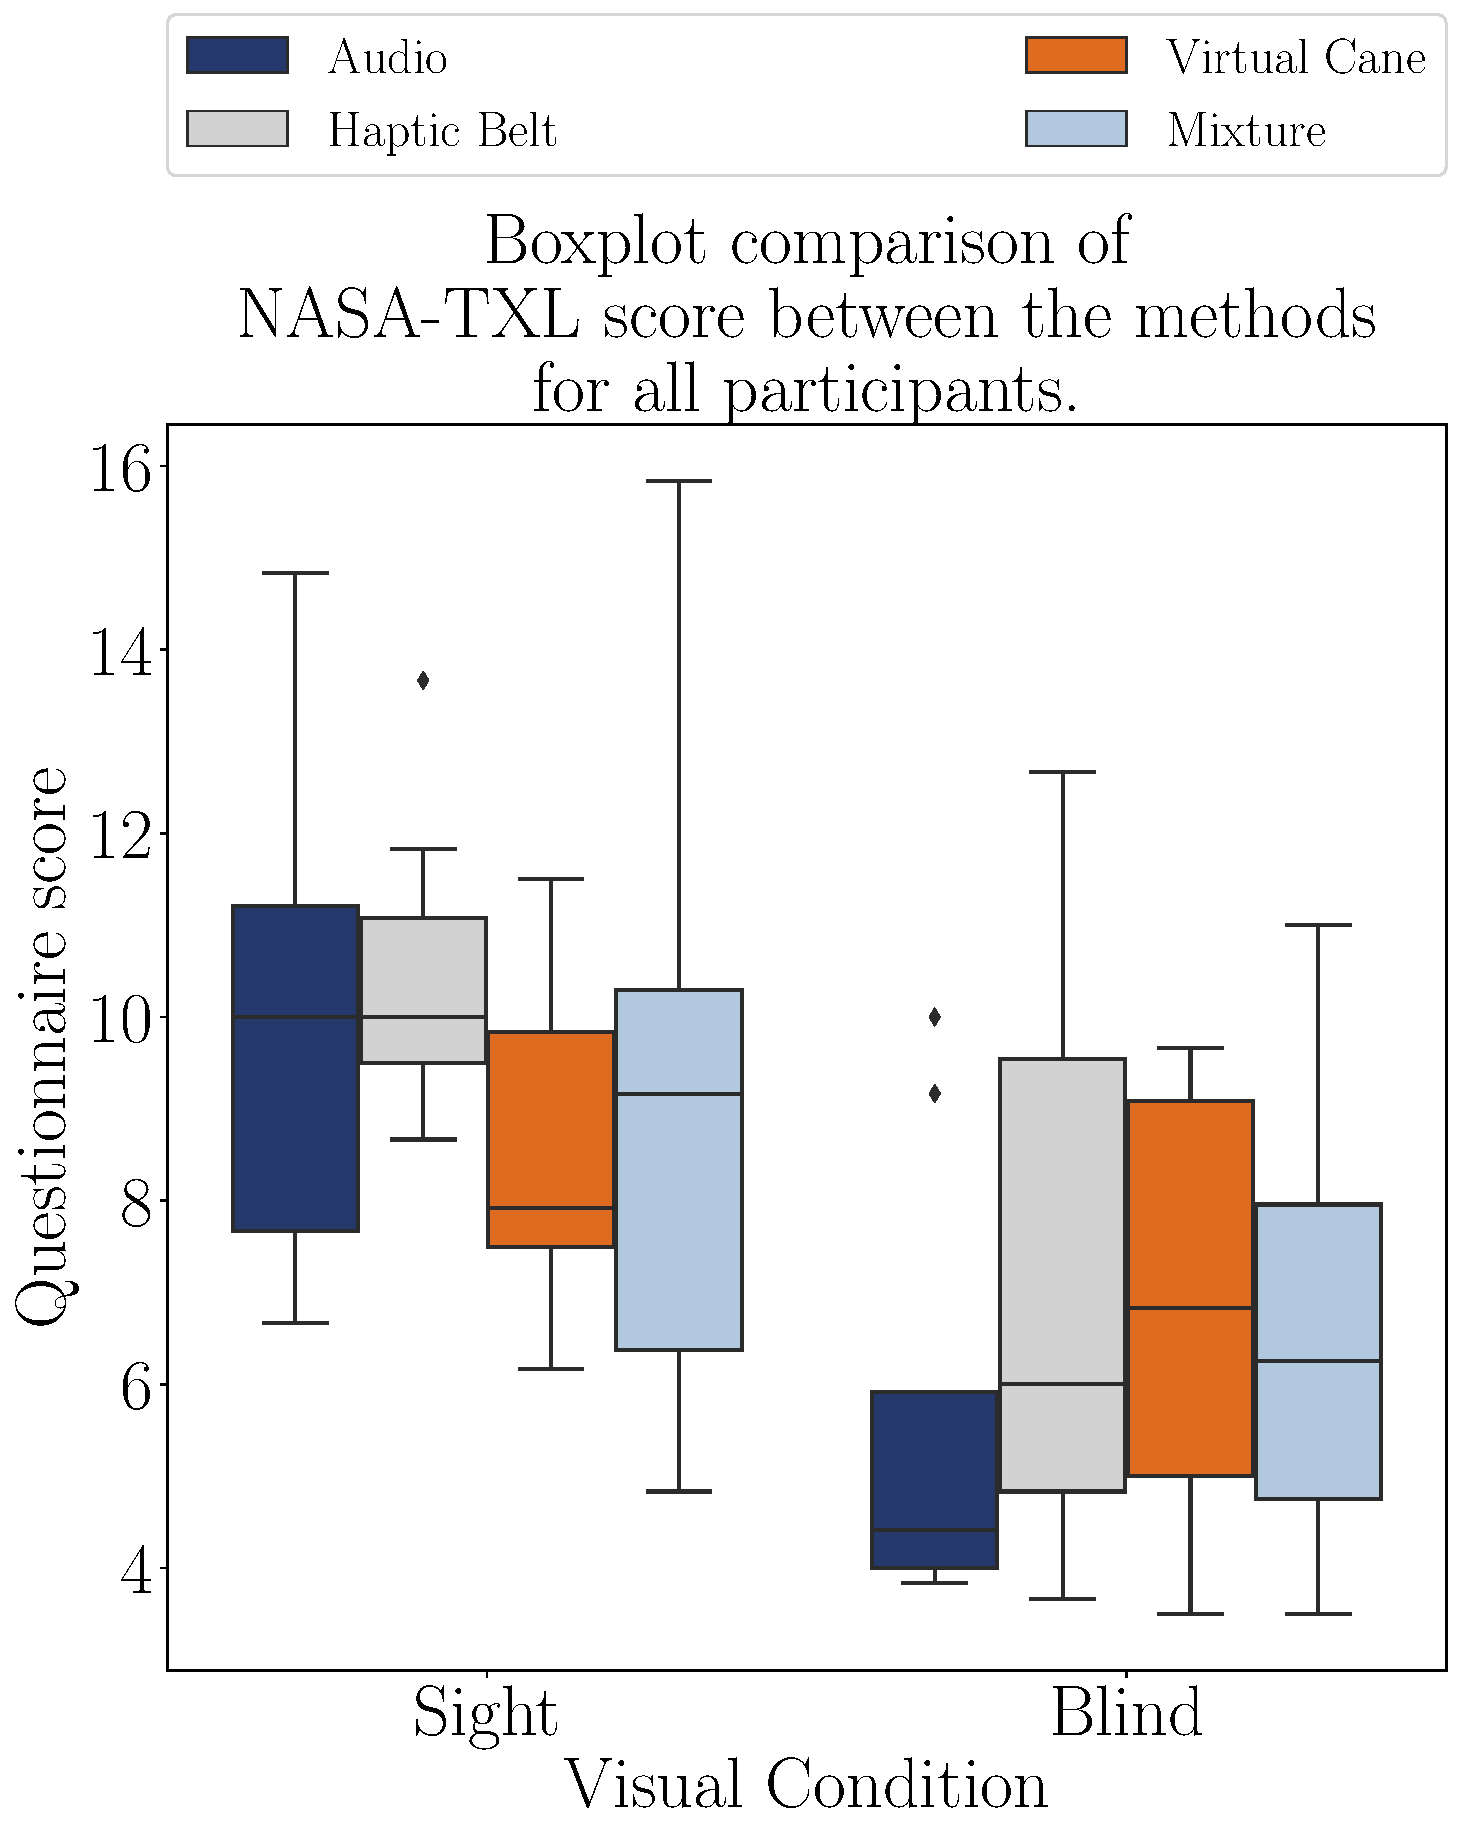
\includegraphics[width = \textwidth]{Resultados/Nasa/Figuras/pdf/boxplot_noBase_nasa_4_scene.pdf}
        \caption{Boxplot of the NASA-TLX score of the participants grouped by the methods.}
        \label{fig:boxplot_noBase_nasa_4_scene}
    \end{minipage}
    \begin{minipage}{0.075\textwidth}
        \hfill
    \end{minipage}
    \begin{minipage}{0.45\textwidth}
        \centering
        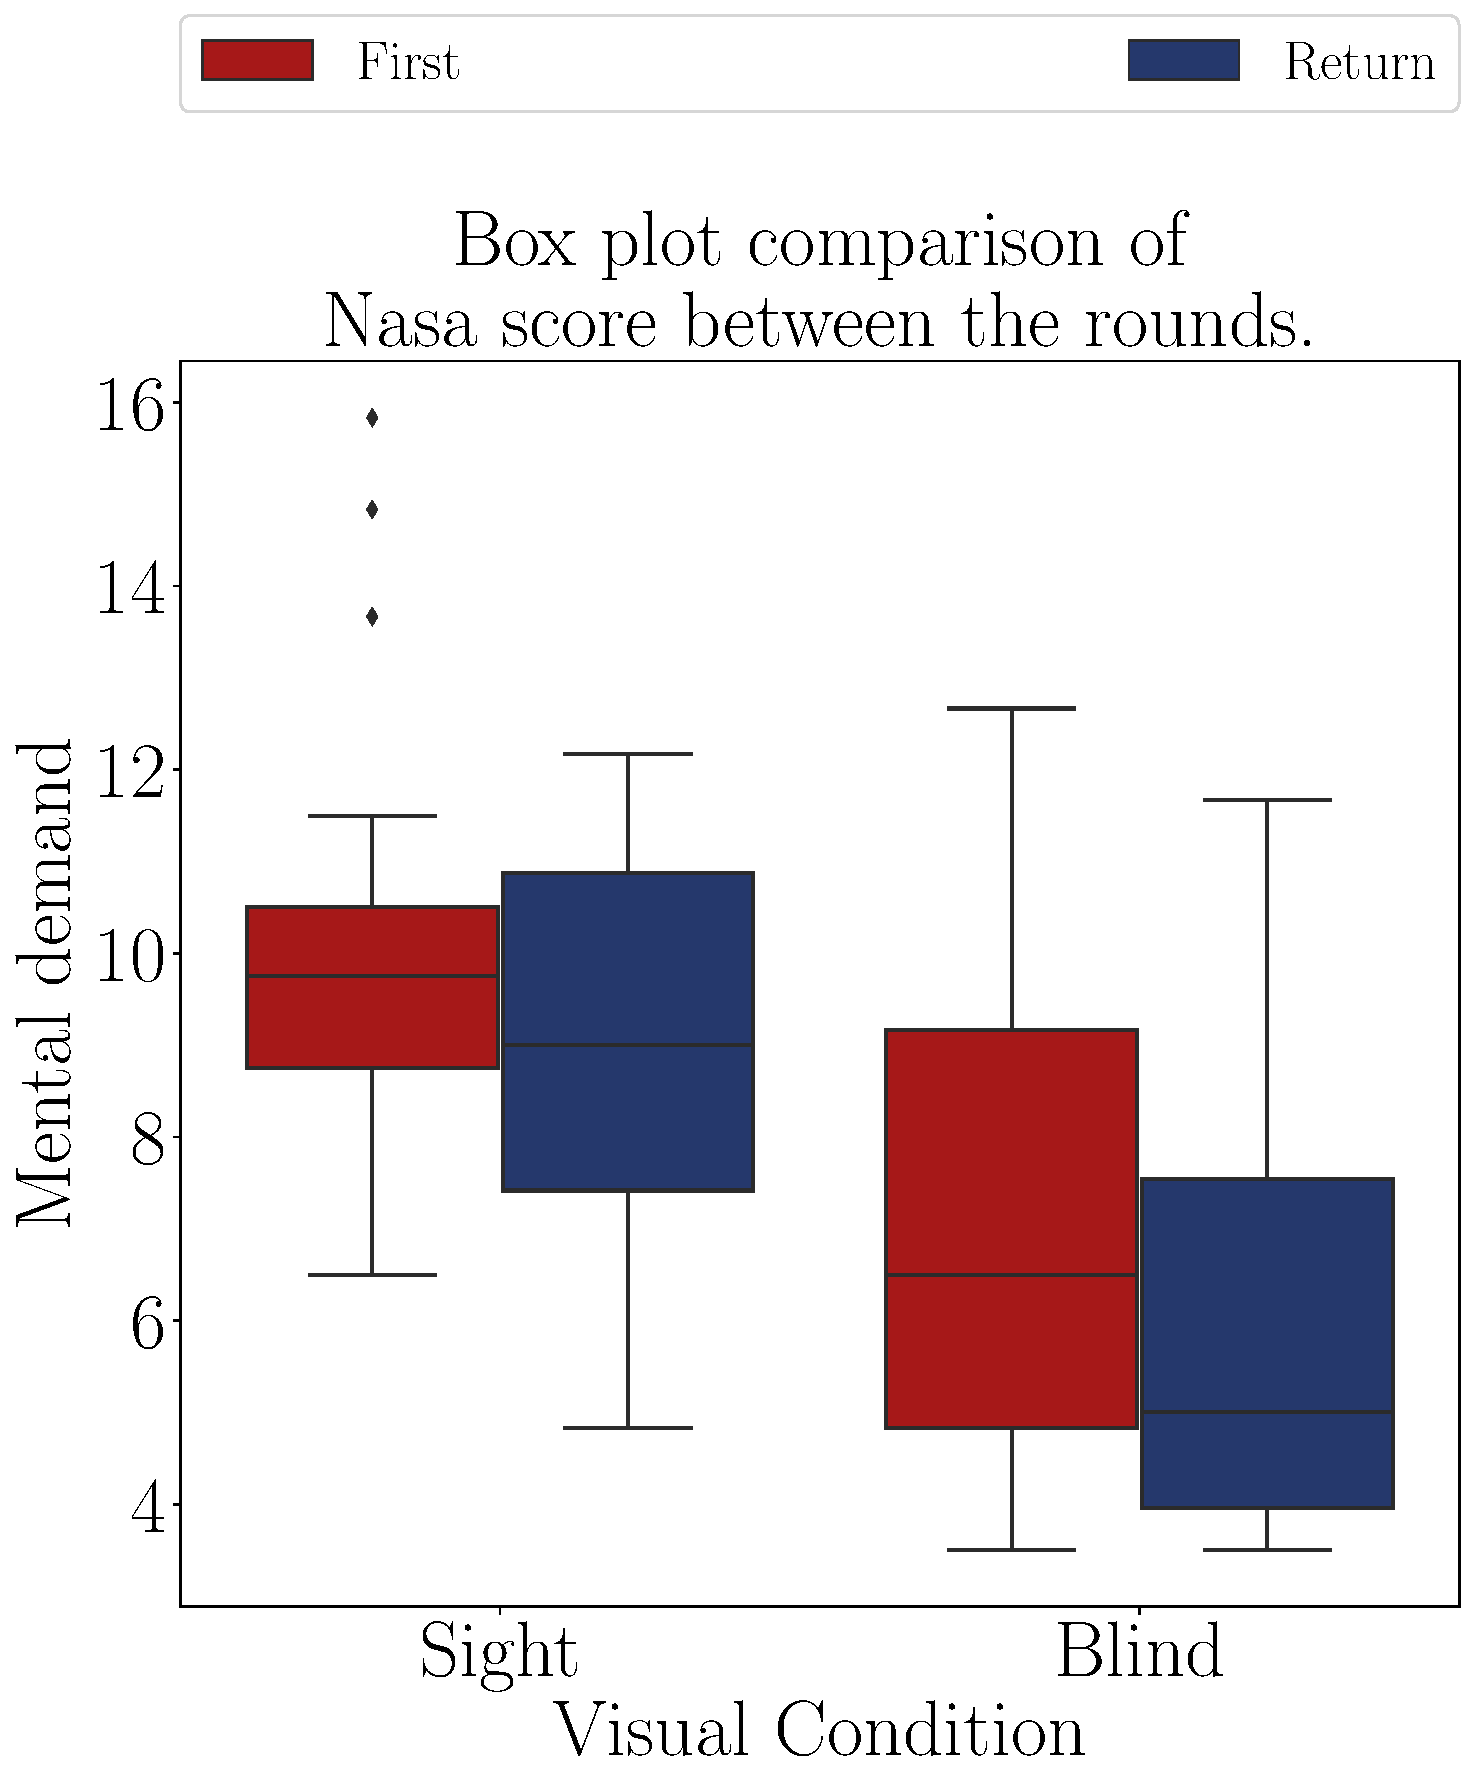
\includegraphics[width = \textwidth]{Resultados/Nasa/Figuras/pdf/boxplot_noBase_nasa_4_rounds.pdf}
        \caption{Boxplot of the NASA-TLX score of the participants grouped by the rounds.}
        \label{fig:boxplot_noBase_nasa_4_rounds}
    \end{minipage}
\end{figure}

Figures \ref{fig:qqplot_nasa_avg_two_way_sight} and \ref{fig:residplot_nasa_avg_two_way_sight} bring the QQ plot and residual distribution of the data from sighted participants, showing that ANOVA can be used. The p-values for both groups are presented in Table \ref{tab:blocanova_nasa_avg_two_way_blind_sight}. It confirms the influence of the round for both sighted and blind people. In the case of the methods, the p-value of blind is lower than the threshold of 0.5, while that of sighted is slightly higher.

\begin{table}[!thb]
    \caption{Anova p-value for the NASA-TLX score on each method}
    \label{tab:blocanova_nasa_avg_two_way_blind_sight}
    \begin{minipage}{0.45\textwidth}
        \subcaption{Blind participants}
        
\centering
\begin{tabular}{ll}
\toprule
          Source & P-Value \\
\midrule
    \    Methods & 0.029** \\
     \    Rounds & 0.022** \\
\    Interaction &   0.814 \\
\bottomrule
\end{tabular}

    \end{minipage}
    \begin{minipage}{0.45\textwidth}
        \subcaption{Sight participants}
        
\centering
\begin{tabular}{ll}
\toprule
          Source & P-Value \\
\midrule
    \    Methods &   0.086 \\
     \    Rounds & 0.034** \\
\    Interaction &   0.688 \\
\bottomrule
\end{tabular}
    
    \end{minipage}
\end{table}


\begin{figure}[!htb]
    \centering
    %\vspace{-15.0cm}
    \begin{minipage}{0.45\textwidth}
        \centering
        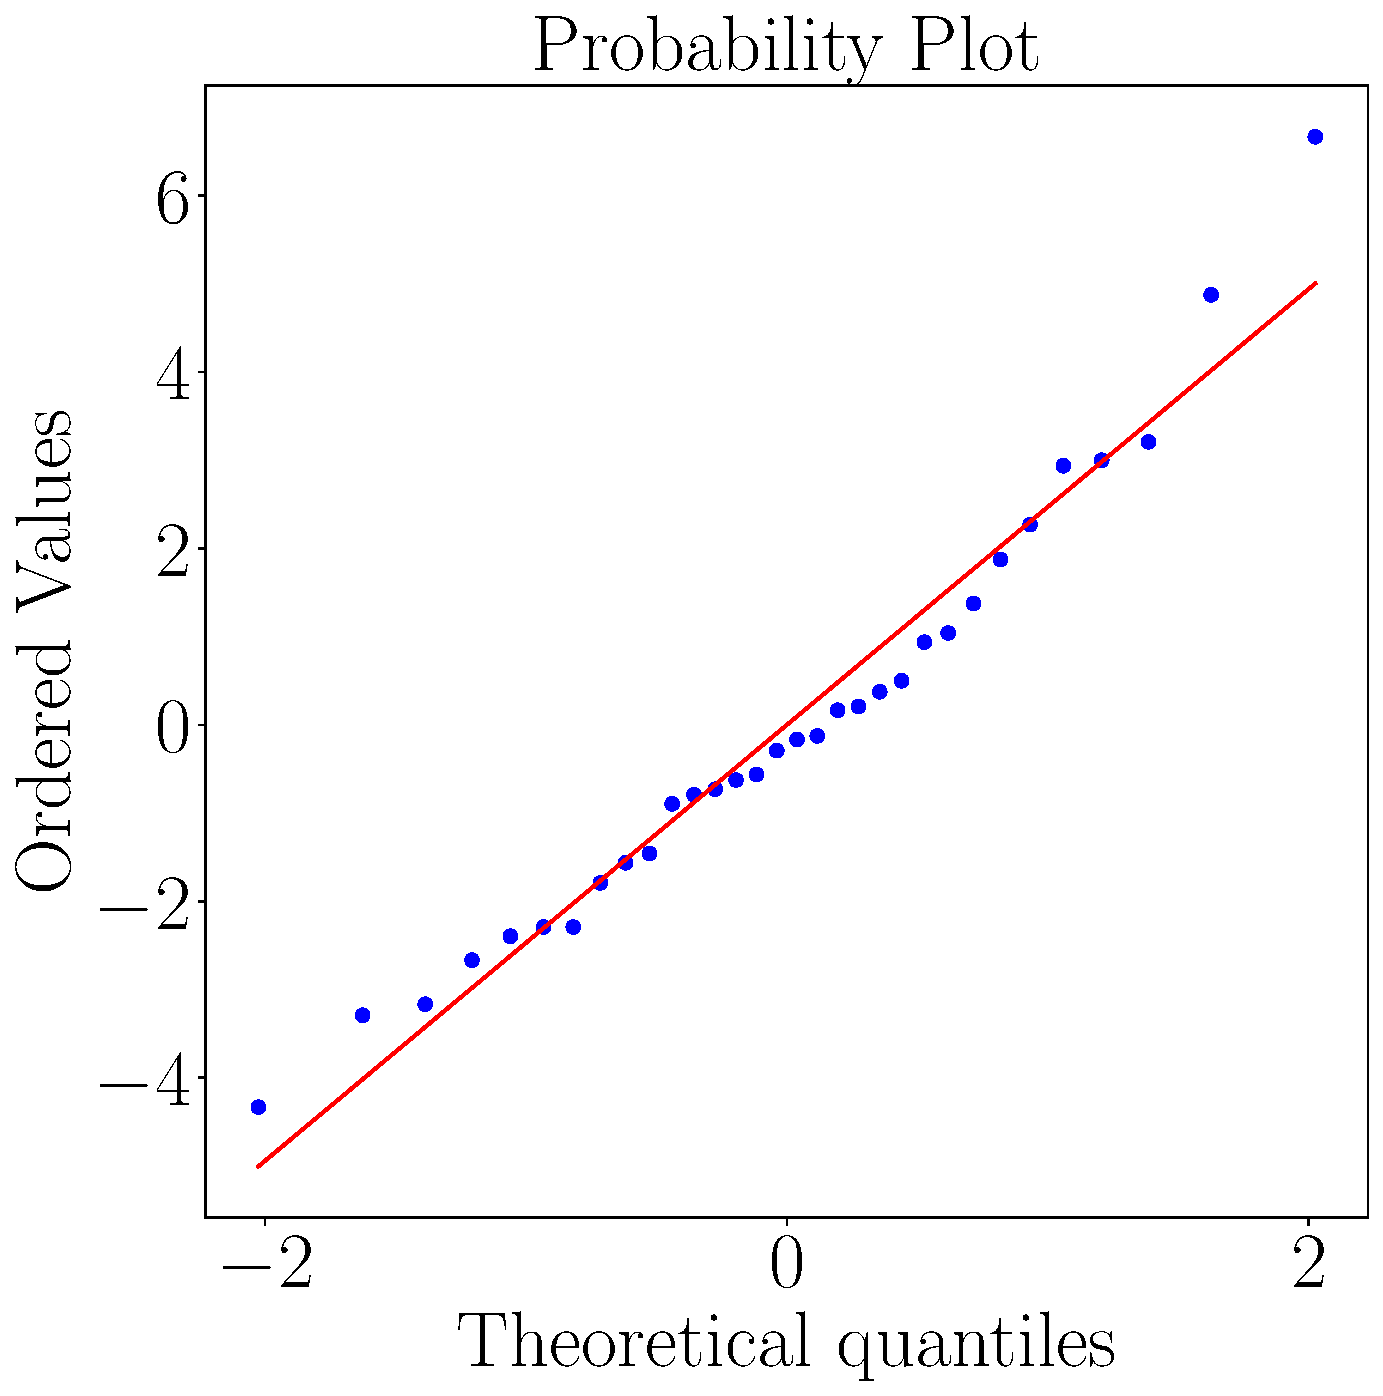
\includegraphics[width = \textwidth]{Resultados/Nasa/Figuras/pdf/qqplot_nasa_avg_two_way_sight.pdf}
        \caption{QQ plot of the NASA-TLX score of the sight participants on each method.}
        \label{fig:qqplot_nasa_avg_two_way_sight}
    \end{minipage}
    \begin{minipage}{0.075\textwidth}
        \hfill
    \end{minipage}
    \begin{minipage}{0.45\textwidth}
        \centering
        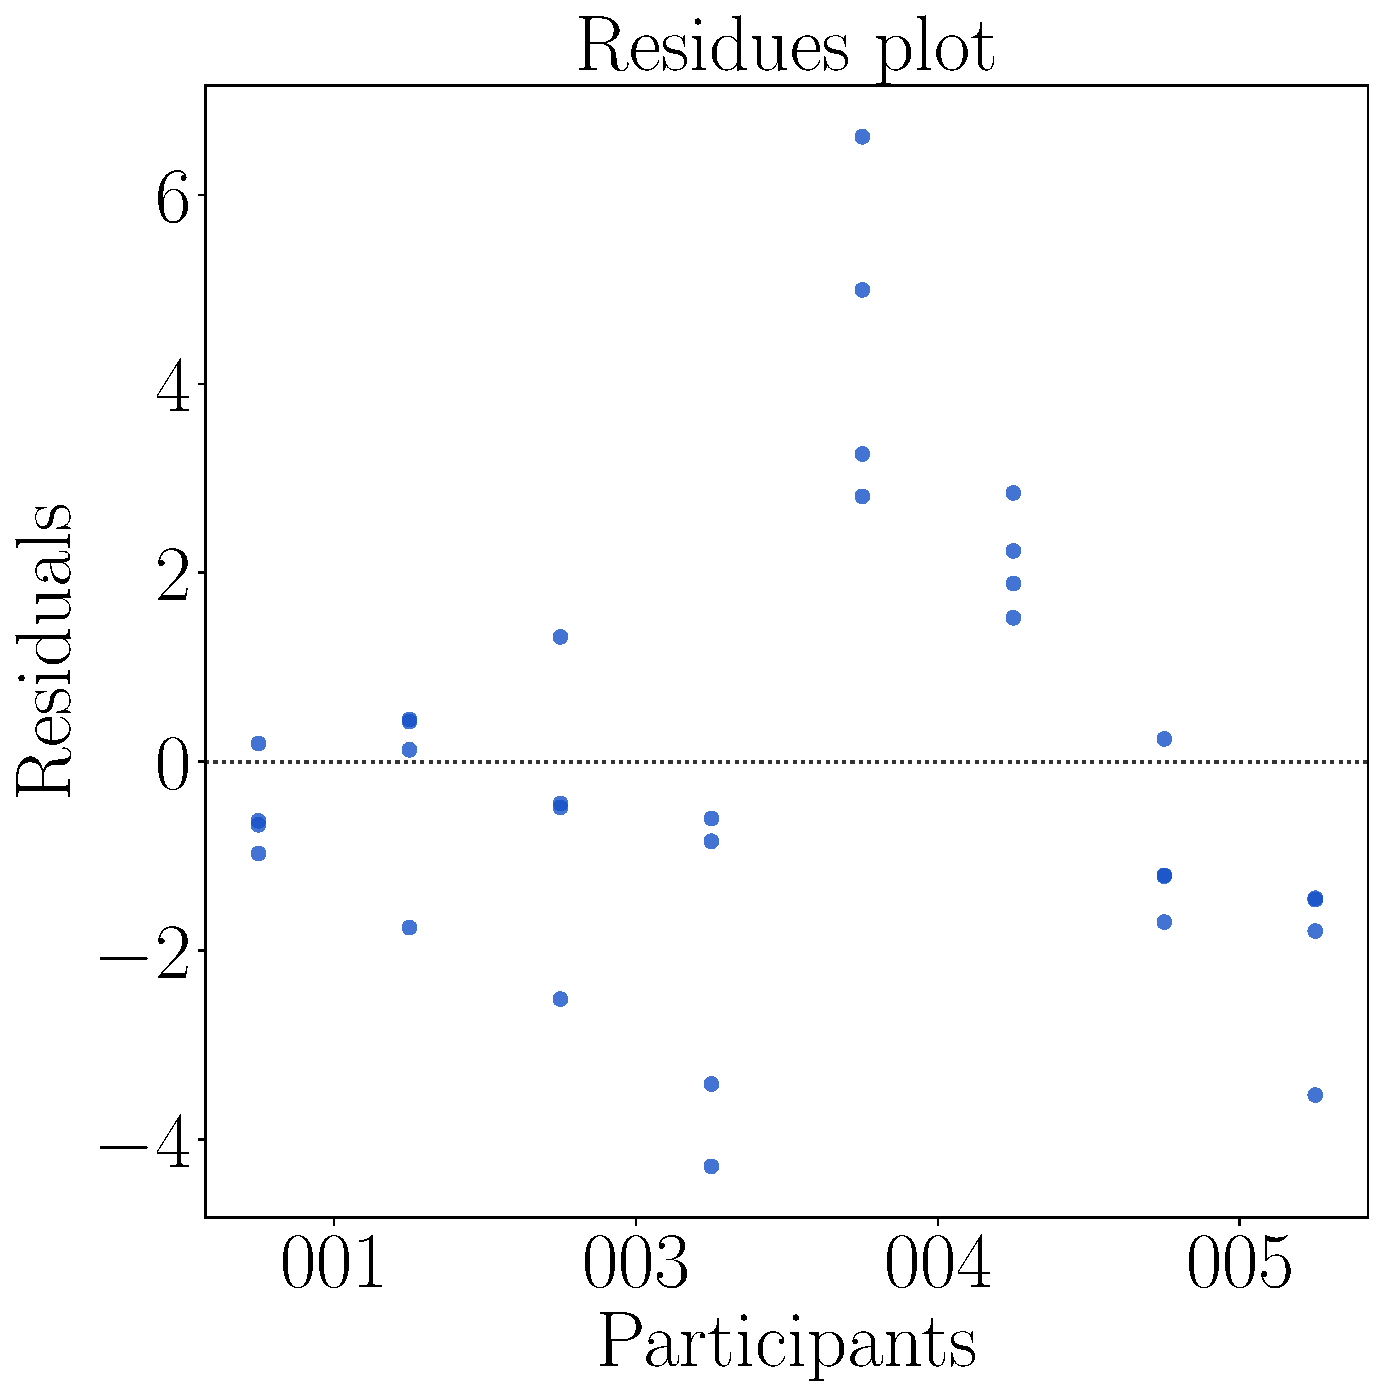
\includegraphics[width = \textwidth]{Resultados/Nasa/Figuras/pdf/residplot_nasa_avg_two_way_sight.pdf}
        \caption{Residual plot of the NASA-TLX score the sight participants on each method.}
        \label{fig:residplot_nasa_avg_two_way_sight}
    \end{minipage}
\end{figure}

\FloatBarrier